\documentclass[11pt]{article}
\usepackage[margin=0.9in]{geometry}
\usepackage{amsmath,amssymb,booktabs,array}
\usepackage{tikz}
\usetikzlibrary{arrows.meta,positioning,calc,fit}
\setlength{\parindent}{0pt}
\setlength{\parskip}{4pt}

\tikzset{
  st/.style={draw, rounded corners=2pt, inner sep=3pt, minimum width=1.25cm, font=\small},
  ghost/.style={st, dashed, draw=gray!60, text=gray!60},
  ar/.style={-{Stealth[length=2mm]}, thin},
  lab/.style={font=\scriptsize, fill=white, inner sep=1pt},
}

\title{SCUDEM XI, Problem B: model notes}
\author{Team 26100}
\date{November 7, 2026}

\begin{document}
\maketitle

\textit{Note: I had Claude help with the \LaTeX\ and the diagrams. I figured this would be more readable than my handwritten notes.}

Two spider monkeys, A and B, forage in the same forest and can tip each other off about food.
State = what mode each monkey is in, not where it is. Modes: \textbf{S} searching,
\textbf{T} traveling to a tip, \textbf{E$_a$} eating alone, \textbf{E$_s$} eating a shared patch
(only together). Every arrow is a rate; the probability of each pair state obeys
$\frac{d}{dt}P = \text{flow in} - \text{flow out}$.

\section{Parameters}

\subsection*{Chosen}
\renewcommand{\arraystretch}{1.15}
\begin{tabular}{>{$}l<{$} l l l}
\toprule
 & meaning & units & default \\
\midrule
\multicolumn{4}{l}{\textit{environment}}\\
A & forest area & $L^2$ & $100^2$ \\
n & number of good patches & count & 13 \\
w & patch width (gaussian $\sigma$) & $L$ & 3 \\
\text{amp} & peak food density of a fresh patch & food$/L^2$ & 10 \\
m & density a monkey notices & food$/L^2$ & 0.5 \\
\kappa & rate a patch vanishes on its own (rot, fall, competitors) & $T^{-1}$ & 0.01 \\
\multicolumn{4}{l}{\textit{monkey}}\\
v & travel speed & $L/T$ & 0.5 \\
r & vision radius & $L$ & 2 \\
c & eat rate & $T^{-1}$ & 0.03 \\
d & separation of the pair & $L$ & 10 (swept) \\
\multicolumn{4}{l}{\textit{communication}}\\
C & channel capacity & bits$/T$ & 10 \\
b & bits per tip & bits & 10 \\
\sigma_0 & tip blur per unit distance & none (rad) & 0.05 \\
R_c & contact range & $L$ & 30 \\
p_A,\,p_B & accuracy of tips A, B send ($1-p_{\text{lie}}$) & prob. & 1 \\
\phi & forgiveness rate (a feud lasts $1/\phi$) & $T^{-1}$ & $1/1500$ \\
\bottomrule
\end{tabular}

\subsection*{Derived}
\begin{tabular}{>{$}l<{$} >{$}l<{$} l l l}
\toprule
 & \text{formula} & meaning & units & at defaults \\
\midrule
\lambda & 2rv\,n/A & discovery rate while searching & $T^{-1}$ & 0.0026 \\
\mu & c/\ln(\text{amp}/m) & patch depletion rate, one eater & $T^{-1}$ & 0.0100 \\
F & 2\pi\,\text{amp}\,w^2 & food in a fresh patch & food & 565 \\
e & \mu F & intake rate while eating & food$/T$ & 5.66 \\
c(d) & 1 \text{ if } d\le R_c \text{ else } 0 & contact factor & none & 1 \\
o(d) & \frac1n + \left(1-\frac1n\right)e^{-d/(r+w)} & overlap: chance a find is in shared ground & none & 0.20 \\
a_\ell & \max\!\left(A\,2^{-b},\ \pi(\sigma_0 d)^2\right) & area left to search after a tip & $L^2$ & 9.77 \\
\tau & d/v + a_\ell/(2rv) & mean trip time & $T$ & 24.9 \\
\nu & C/b & tip rate & $T^{-1}$ & 1 \\
\bottomrule
\end{tabular}

Notes: a patch with one eater ends at rate $\mu+\kappa$ (eaten out or vanishes); a shared patch at $2\mu+\kappa$.
$\mu$ solves $\text{amp}\,e^{-ct}=m$ for the patch lifetime. $F$ is the polar integral of the gaussian.
$\lambda$ is the swept strip $2r$ wide. Each bit halves the area left to search, but never below the blur circle.

\section{The 9-state model}

States: (S,S), (S,E$_a$), (E$_a$,S), (E$_a$,E$_a$), (T,E$_a$), (E$_a$,T), (T,S), (S,T), (E$_s$,E$_s$),
written (A's mode, B's mode).

\subsection*{A's arrows (B mirrors, with $p_A \leftrightarrow p_B$)}
\begin{tabular}{l l >{$}l<{$} l}
\toprule
from & to & \text{rate} & \\
\midrule
(S,S) & (E$_a$,S) & \lambda(1-o) & A finds its own patch \\
(S,S) & (E$_s$,E$_s$) & \lambda o & find in shared ground, both eat (one arrow) \\
(S,E$_a$) & (E$_a$,E$_a$) & \lambda(1-o) & A finds its own patch \\
(S,E$_a$) & (E$_s$,E$_s$) & \lambda o & A stumbles onto B's patch \\
(S,E$_a$) & (T,E$_a$) & \nu c(d) & B tips A \\
(T,E$_a$) & (E$_s$,E$_s$) & p_B/\tau & true tip, they share \\
(T,E$_a$) & (S,E$_a$) & (1-p_B)/\tau & false tip, nothing there \\
(T,E$_a$) & (T,S) & (\mu+\kappa) & B's patch ends while A is en route \\
(T,S) & (S,S) & 1/\tau & A arrives, patch gone \\
(T,S) & (T,E$_a$) & \lambda & B finds a new patch and re-tips \\
(E$_a$,S) & (S,S) & (\mu+\kappa) & A's patch ends \\
(E$_a$,E$_a$) & (S,E$_a$) & (\mu+\kappa) & A's patch ends \\
(E$_s$,E$_s$) & (S,S) & (2\mu+\kappa) & shared patch ends (one arrow) \\
\bottomrule
\end{tabular}

\begin{center}
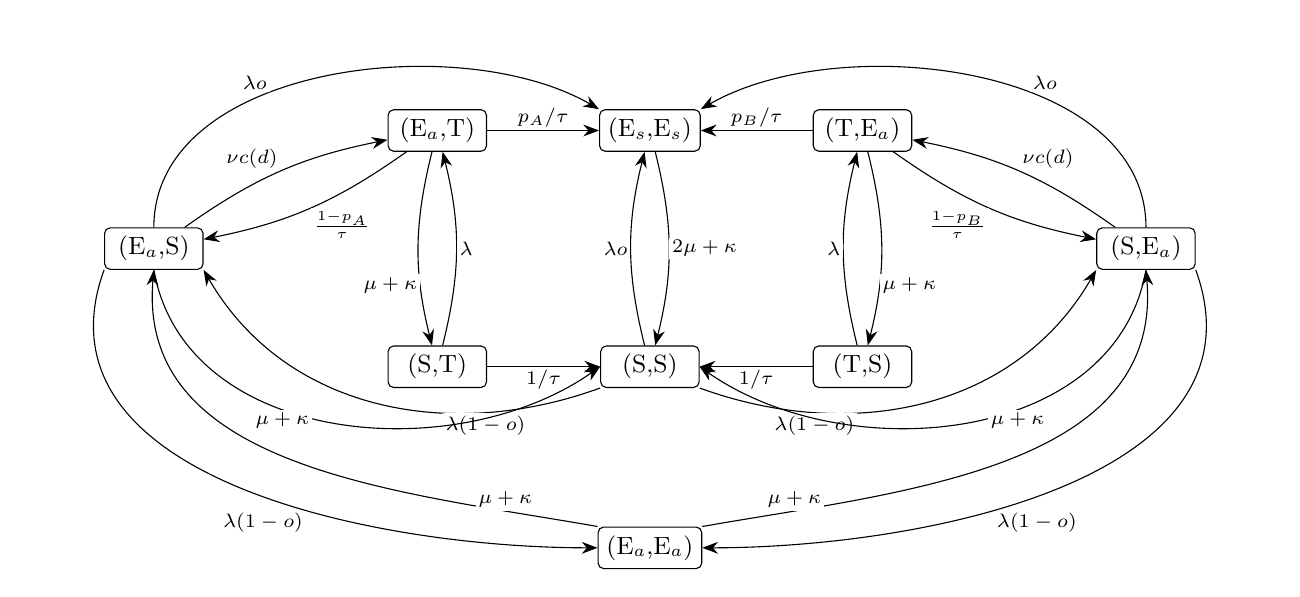
\begin{tikzpicture}[x=1cm,y=1cm]
  % top row: eating together, and on the way to a tip
  \node[st] (ET) at (-2.7,3) {(E$_a$,T)};
  \node[st] (Es) at (0,3) {(E$_s$,E$_s$)};
  \node[st] (TE) at (2.7,3) {(T,E$_a$)};
  % sides: one eating, one searching
  \node[st] (ES) at (-6.3,1.5) {(E$_a$,S)};
  \node[st] (SE) at (6.3,1.5) {(S,E$_a$)};
  % bottom row: searching
  \node[st] (ST) at (-2.7,0) {(S,T)};
  \node[st] (SS) at (0,0) {(S,S)};
  \node[st] (TS) at (2.7,0) {(T,S)};
  \node[st] (EE) at (0,-2.3) {(E$_a$,E$_a$)};
  % center column
  \draw[ar] (SS) to[bend left=14] node[lab,left] {$\lambda o$} (Es);
  \draw[ar] (Es) to[bend left=14] node[lab,right] {$2\mu+\kappa$} (SS);
  % tips: send, true, false
  \draw[ar] (ES) to[bend left=12] node[lab,above left] {$\nu c(d)$} (ET);
  \draw[ar] (ET) to[bend left=12] node[lab,below right,pos=0.5] {$\frac{1-p_A}{\tau}$} (ES);
  \draw[ar] (SE) to[bend right=12] node[lab,above right] {$\nu c(d)$} (TE);
  \draw[ar] (TE) to[bend right=12] node[lab,below left,pos=0.5] {$\frac{1-p_B}{\tau}$} (SE);
  \draw[ar] (ET) -- node[lab,above] {$p_A/\tau$} (Es);
  \draw[ar] (TE) -- node[lab,above] {$p_B/\tau$} (Es);
  % tipper's patch ends en route; re-tip; stale arrival
  \draw[ar] (ET) to[bend right=14] node[lab,left,pos=0.7] {$\mu+\kappa$} (ST);
  \draw[ar] (ST) to[bend right=14] node[lab,right] {$\lambda$} (ET);
  \draw[ar] (TE) to[bend left=14] node[lab,right,pos=0.7] {$\mu+\kappa$} (TS);
  \draw[ar] (TS) to[bend left=14] node[lab,left] {$\lambda$} (TE);
  \draw[ar] (ST) -- node[lab,below] {$1/\tau$} (SS);
  \draw[ar] (TS) -- node[lab,below] {$1/\tau$} (SS);
  % stumble onto the partner's patch (over the top)
  \draw[ar] (ES.north) to[out=90,in=150,looseness=0.9] node[lab,above left,pos=0.4] {$\lambda o$} (Es.north west);
  \draw[ar] (SE.north) to[out=90,in=30,looseness=0.9] node[lab,above right,pos=0.4] {$\lambda o$} (Es.north east);
  % searching <-> one eating (under the T boxes)
  \draw[ar] (SS.south west) to[out=200,in=-60] node[lab,pos=0.25,below] {$\lambda(1-o)$} (ES.south east);
  \draw[ar] (ES.south) to[out=-80,in=215] node[lab,pos=0.4,below] {$\mu+\kappa$} (SS.west);
  \draw[ar] (SS.south east) to[out=-20,in=240] node[lab,pos=0.25,below] {$\lambda(1-o)$} (SE.south west);
  \draw[ar] (SE.south) to[out=260,in=-35] node[lab,pos=0.4,below] {$\mu+\kappa$} (SS.east);
  % one eating <-> both eating alone (bottom)
  \draw[ar] (ES.south west) to[out=-110,in=180] node[lab,pos=0.6,below left] {$\lambda(1-o)$} (EE.west);
  \draw[ar] (EE.north west) to[out=170,in=-95] node[lab,pos=0.15,above] {$\mu+\kappa$} (ES.south);
  \draw[ar] (SE.south east) to[out=-70,in=0] node[lab,pos=0.6,below right] {$\lambda(1-o)$} (EE.east);
  \draw[ar] (EE.north east) to[out=10,in=-85] node[lab,pos=0.15,above] {$\mu+\kappa$} (SE.south);
\end{tikzpicture}
\end{center}

\subsection*{Equations}
$P_{XY}$ is the probability of state (X,Y): first letter is A's mode, second is B's, and E means E$_a$
(so $P_{SE} = P(\text{S},\text{E}_a)$). $P_{E_sE_s}$ is the shared state.
{\small
\begin{align*}
\dot P_{SS} &= (\mu+\kappa)(P_{SE}+P_{ES}) + (2\mu+\kappa) P_{E_sE_s} + \tfrac1\tau(P_{ST}+P_{TS}) - \lambda(2-o)\,P_{SS}\\
\dot P_{SE} &= \lambda(1-o)P_{SS} + (\mu+\kappa) P_{EE} + \tfrac{1-p_B}{\tau}P_{TE} - (\lambda + \nu c(d) + \mu+\kappa)P_{SE}\\
\dot P_{ES} &= \lambda(1-o)P_{SS} + (\mu+\kappa) P_{EE} + \tfrac{1-p_A}{\tau}P_{ET} - (\lambda + \nu c(d) + \mu+\kappa)P_{ES}\\
\dot P_{EE} &= \lambda(1-o)(P_{SE}+P_{ES}) - 2(\mu+\kappa)P_{EE}\\
\dot P_{TE} &= \nu c(d)\,P_{SE} + \lambda P_{TS} - (\tfrac1\tau + \mu+\kappa)P_{TE}\\
\dot P_{ET} &= \nu c(d)\,P_{ES} + \lambda P_{ST} - (\tfrac1\tau + \mu+\kappa)P_{ET}\\
\dot P_{TS} &= (\mu+\kappa) P_{TE} - (\tfrac1\tau + \lambda)P_{TS}\\
\dot P_{ST} &= (\mu+\kappa) P_{ET} - (\tfrac1\tau + \lambda)P_{ST}\\
\dot P_{E_sE_s} &= \lambda o\,(P_{SS}+P_{SE}+P_{ES}) + \tfrac{p_B}{\tau}P_{TE} + \tfrac{p_A}{\tau}P_{ET} - (2\mu+\kappa) P_{E_sE_s}
\end{align*}}
This is linear, $\dot P = PQ$, and the steady state solves $PQ = 0$ with $\sum P = 1$.

\textbf{Readout.} Intake of A $= e\cdot P(\text{A eating}) = e\,(P_{ES}+P_{EE}+P_{ET}+P_{E_sE_s})$; B mirrors.
\textbf{Silent} (no communication) = same chain with channel capacity $C = 0$, so the tip rate $\nu = C/b = 0$
and no T state is ever reached. (Careful: $C$ is channel capacity, $c$ is eat rate, and $c(d)$ is the contact factor.)

\section{The 14-state model: adding a feud}

This model is best understood as an extension of the 9-state model in Section 2, which is why both are included:
everything in Section 2 still holds, and the feud adds one mechanism on top.

A false tip (A arrives, nothing there, B still eating) starts a \textbf{feud}: no tips until forgiven.
The feud is a copy of the 9-state diagram with the tip arrows $\nu c(d)$ set to 0. The T boxes become
unreachable, leaving 5 boxes; this is just the silent model.
Two changes connect the copies:
\begin{itemize}\itemsep0pt
\item the false-tip arrow $(T,E_a)\xrightarrow{(1-p_B)/\tau}(S,E_a)$ now lands in the feud copy $(S,E_a)_f$ (mirror for A);
\item every feud box returns to its twin at rate $\phi$.
\end{itemize}
The receiver can't tell a lie from an honest mistake, so both start feuds.

\begin{center}
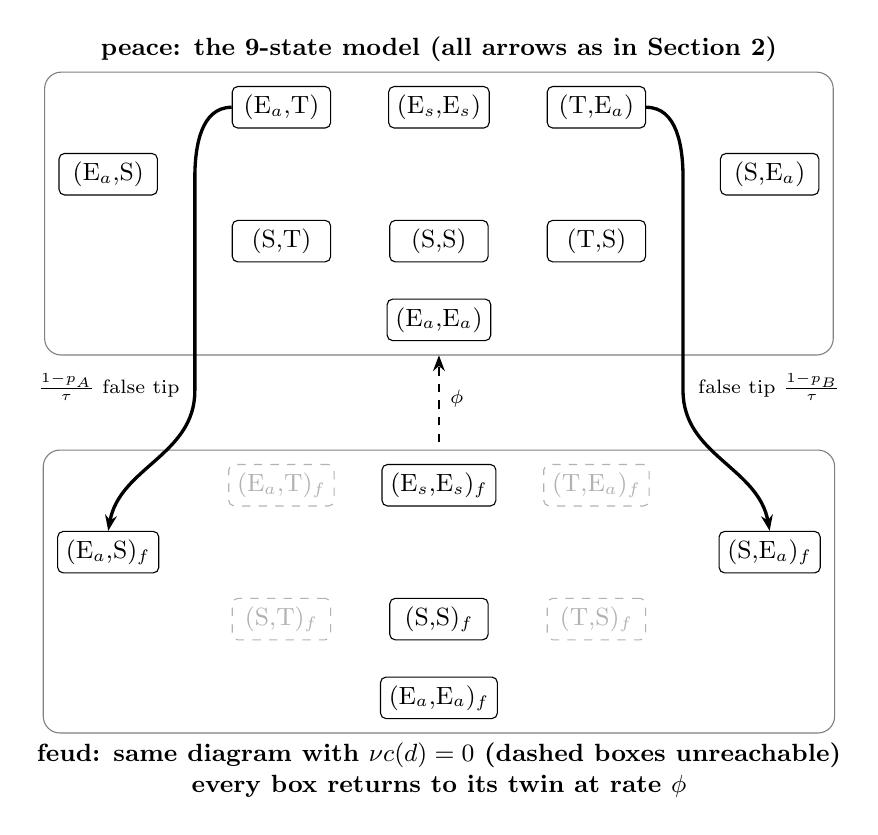
\begin{tikzpicture}[x=1cm,y=1cm]
  \node[st] (ET) at (-2.0,6.50) {(E$_a$,T)};
  \node[st] (Es) at (0,6.50) {(E$_s$,E$_s$)};
  \node[st] (TE) at (2.0,6.50) {(T,E$_a$)};
  \node[st] (ES) at (-4.2,5.65) {(E$_a$,S)};
  \node[st] (SE) at (4.2,5.65) {(S,E$_a$)};
  \node[st] (ST) at (-2.0,4.80) {(S,T)};
  \node[st] (SS) at (0,4.80) {(S,S)};
  \node[st] (TS) at (2.0,4.80) {(T,S)};
  \node[st] (EE) at (0,3.80) {(E$_a$,E$_a$)};
  \node[draw, rounded corners=6pt, gray, fit=(ES)(SE)(ET)(EE), inner sep=5pt, label={[font=\small\bfseries]above:peace: the 9-state model (all arrows as in Section 2)}] {};
  \node[ghost] (ETf) at (-2.0,1.70) {(E$_a$,T)$_f$};
  \node[st] (Esf) at (0,1.70) {(E$_s$,E$_s$)$_f$};
  \node[ghost] (TEf) at (2.0,1.70) {(T,E$_a$)$_f$};
  \node[st] (ESf) at (-4.2,0.85) {(E$_a$,S)$_f$};
  \node[st] (SEf) at (4.2,0.85) {(S,E$_a$)$_f$};
  \node[ghost] (STf) at (-2.0,0.00) {(S,T)$_f$};
  \node[st] (SSf) at (0,0.00) {(S,S)$_f$};
  \node[ghost] (TSf) at (2.0,0.00) {(T,S)$_f$};
  \node[st] (EEf) at (0,-1.00) {(E$_a$,E$_a$)$_f$};
  \node[draw, rounded corners=6pt, gray, fit=(ESf)(SEf)(ETf)(EEf), inner sep=5pt, label={[font=\small\bfseries, align=center]below:{feud: same diagram with $\nu c(d)=0$ (dashed boxes unreachable)\\every box returns to its twin at rate $\phi$}}] {};
  % false tips into the feud
  \draw[ar, very thick] (TE.east) to[out=0,in=90] (3.1,5.6) -- (3.1,2.9) to[out=-90,in=100] (SEf.north);
  \node[lab, anchor=west] at (3.25,2.95) {false tip $\frac{1-p_B}{\tau}$};
  \draw[ar, very thick] (ET.west) to[out=180,in=90] (-3.1,5.6) -- (-3.1,2.9) to[out=-90,in=80] (ESf.north);
  \node[lab, anchor=east] at (-3.25,2.95) {$\frac{1-p_A}{\tau}$ false tip};
  % forgiveness
  \draw[ar, dashed, thick] (0,2.25) -- (0,3.35);
  \node[lab, anchor=west] at (0.1,2.8) {$\phi$};
\end{tikzpicture}
\end{center}

\subsection*{Changes to the equations}
In the 9 peace equations, replace $\frac{1-p_B}{\tau}P_{TE}$ in $\dot P_{SE}$ with $\phi P_{SE,f}$
(and $\frac{1-p_A}{\tau}P_{ET}$ in $\dot P_{ES}$ with $\phi P_{ES,f}$), and add $+\phi P_{X,f}$ to
$\dot P_{SS}$, $\dot P_{EE}$, $\dot P_{E_sE_s}$. The feud copy:
{\small
\begin{align*}
\dot P_{SS,f} &= (\mu+\kappa)(P_{SE,f}+P_{ES,f}) + (2\mu+\kappa) P_{E_sE_s,f} - (\lambda(2-o) + \phi)P_{SS,f}\\
\dot P_{SE,f} &= \lambda(1-o)P_{SS,f} + (\mu+\kappa) P_{EE,f} + \tfrac{1-p_B}{\tau}P_{TE} - (\lambda + \mu+\kappa + \phi)P_{SE,f}\\
\dot P_{ES,f} &= \lambda(1-o)P_{SS,f} + (\mu+\kappa) P_{EE,f} + \tfrac{1-p_A}{\tau}P_{ET} - (\lambda + \mu+\kappa + \phi)P_{ES,f}\\
\dot P_{EE,f} &= \lambda(1-o)(P_{SE,f}+P_{ES,f}) - (2\mu+2\kappa + \phi)P_{EE,f}\\
\dot P_{E_sE_s,f} &= \lambda o\,(P_{SS,f}+P_{SE,f}+P_{ES,f}) - (2\mu+\kappa + \phi)P_{E_sE_s,f}
\end{align*}}
Intake counts eating in both copies. As $\phi\to\infty$ (forgive instantly) this is exactly the 9-state model.

\textbf{Assumptions to state:} all waits are exponential (a trip takes \emph{mean} $\tau$); the environment is
constant ($n$ fixed, since unclaimed patches turn over at rate $\kappa$); the receiver always follows a tip outside a feud.

\end{document}
